\documentclass[a4paper,UKenglish]{lipics-v2016}

\usepackage{microtype}%if unwanted, comment out or use option "draft"

% custom packages
\usepackage{mathpartir}
\usepackage{xspace}
\usepackage{tikz}
\usepackage{wrapfig}
\usepackage{float}

\renewcommand{\TirNameStyle}[1]{\small \textsf{#1}}
\renewcommand{\RightTirNameStyle}[1]{\small \textsf{#1}}

%\graphicspath{{./graphics/}}%helpful if your graphic files are in another directory

\bibliographystyle{plainurl}% the recommended bibstyle

% Author macros::begin %%%%%%%%%%%%%%%%%%%%%%%%%%%%%%%%%%%%%%%%%%%%%%%%
\title{Relating System F and $\lambda$2: A Case Study in Coq, Abella and Beluga}
\titlerunning{Relating System F and $\lambda2$}

%% Please provide for each author the \author and \affil macro, even when authors have the same affiliation, i.e. for each author there needs to be the  \author and \affil macros
\author[1]{Jonas Kaiser}
\author[2]{Brigitte Pientka}
\author[1]{Gert Smolka}
\affil[1]{Saarland University, Saarbrücken, Germany\\
  \texttt{\{jkaiser,smolka\}}@ps.uni-saarland.de}
\affil[2]{School of Computer Science, Montreal, Canada\\
  \texttt{bpientka@cs.mcgill.ca}}
\authorrunning{J. Kaiser, B. Pientka and G. Smolka} %mandatory. First: Use abbreviated first/middle names. Second (only in severe cases): Use first author plus 'et. al.'

\Copyright{Jonas Kaiser, Brigitte Pientka and Gert Smolka}%mandatory, please use full first names. LIPIcs license is "CC-BY";  http://creativecommons.org/licenses/by/3.0/

\subjclass{F.4.1 Mathematical Logic -- Lambda calculus and related systems}% mandatory: Please choose ACM 1998 classifications from http://www.acm.org/about/class/ccs98-html . E.g., cite as "F.1.1 Models of Computation".
\keywords{Pure Type Systems, System F, de Bruijn Syntax, Higher-Order Abstract Syntax, Contextual Reasoning}% mandatory: Please provide 1-5 keywords
% Author macros::end %%%%%%%%%%%%%%%%%%%%%%%%%%%%%%%%%%%%%%%%%%%%%%%%%

%Editor-only macros:: begin (do not touch as author)%%%%%%%%%%%%%%%%%%%%%%%%%%%%%%%%%%
\EventEditors{John Q. Open and Joan R. Acces}
\EventNoEds{2}
\EventLongTitle{2nd International Conference on Formal Structures for Computation and Deduction (FSCD 2017)}
\EventShortTitle{FSCD 2017}
\EventAcronym{FSCD}
\EventYear{2017}
\EventDate{September 3--9, 2017}
\EventLocation{Oxford, United Kingdom}
\EventLogo{}
\SeriesVolume{2}
\ArticleNo{XY}
% Editor-only macros::end %%%%%%%%%%%%%%%%%%%%%%%%%%%%%%%%%%%%%%%%%%%%%%%


%%% Content macros::begin %%%%%%%%%%%%%%%%%%%%%%%%%%%%%%%%%%

% uniform meta space
\newcommand{\ms}{\,}
\newcommand{\mrel}[1]{\mathrel{\ms #1 \ms}}

% Meta-Level Propositions
\newcommand{\Prop}{\ensuremath{\mathsf{PROP}}}
\newcommand{\Nat}{\mathbb{N}}

% Meta-level Symbols and Operators
\newcommand{\dom}[1]{\ensuremath{\textrm{dom($#1$)}}}
\newcommand{\OF}{\mrel{:}}
\newcommand{\mOr}{\mrel{\vee}}
\newcommand{\mAnd}{\mrel{\wedge}}
\newcommand{\mAll}[1]{\ensuremath{\forall} #1.\ms\ms}
\newcommand{\mEx}[1]{\ensuremath{\exists} #1.\ms\ms}
\newcommand{\mExu}[1]{\ensuremath{\exists!} #1.\ms\ms}
\newcommand{\bnfdef}{\mrel{::=}}
\newcommand{\eqdef}{\mrel{:=}}
\newcommand{\set}[1]{\ensuremath{\{#1\}}}

\newcommand{\SysL}{$\lambda$2\xspace}


% Syntactic sorts of the object languages
\newcommand{\TyF}{\ensuremath{\mathsf{Ty_{F}}}}
\newcommand{\TmF}{\ensuremath{\mathsf{Tm_{F}}}}
\newcommand{\TmL}{\ensuremath{\mathsf{Tm_{\lambda}}}}

\newcommand{\TyCtxF}{\ensuremath{\mathsf{C_{F}^{ty}}}}
\newcommand{\TmCtxF}{\ensuremath{\mathsf{C_{F}^{tm}}}}
\newcommand{\CtxL}{\ensuremath{\mathsf{C_{\lambda}}}}


% Generic type-system judgement predicates
\newcommand{\istyFpr}{\ensuremath{\mathsf{isty_{F}}}}
\newcommand{\typingFpr}{\ensuremath{\mathsf{ofty_{F}}}}
\newcommand{\typingLpr}{\ensuremath{\mathsf{ofty_{\lambda}}}}

% Judgements
\newcommand{\ty}{\mathsf{ty}}
\newcommand{\tm}{\mathsf{tm}}
\newcommand{\of}{\ensuremath{\!:\!}}
\newcommand{\cc}[2]{#1;#2} % compound System F contexts
\makeatletter
\newcommand{\raisemath}[1]{\mathpalette{\raisem@th{#1}}}
\newcommand{\raisem@th}[3]{\raisebox{#1}{\ensuremath{#2#3}}}
\makeatother
\newcommand{\tsAnnot}[2]{\vdash\hspace{-.7em}^{\raisemath{1.5pt}{\scriptscriptstyle{#2}}}_{\raisemath{0.3pt}{\scriptscriptstyle{#1}}}} % note: wrap instances in \mathbin
\newcommand{\cts}[2]{\ensuremath{(\,#1 #2 {})}} % context + turnstile for CMs
\newcommand{\tfF}{\tsAnnot{\mathsf{F}}{\ty}}  % for type formation judgement
\newcommand{\tyF}{\tsAnnot{\mathsf{F}}{\tm}}  % for typing judgement
\newcommand{\istyF}[2]{\ensuremath{{#1} \mathrel{\tfF} #2}}
\newcommand{\typingF}[3]{\ensuremath{{#1} \mathrel{\tyF} #2 \OF #3}}
\newcommand{\tyL}{\tsAnnot{\lambda}{}} % for typing judgement
\newcommand{\typingL}[3]{\ensuremath{{#1} \mathrel{\tyL} #2 \OF #3}}
\newcommand{\inL}{\mrel{\in_{\lambda}}}
\newcommand{\tfP}{\tsAnnot{\mathsf{P}}{\ty}}  % for type formation judgement
\newcommand{\istyFh}[1]{\ensuremath{#1\ms\mathsf{ty}}}
\newcommand{\typingFh}[2]{\ensuremath{#1 \mathbin{:_{F}} #2}}
\newcommand{\sortLh}[1]{\ensuremath{\mathcal{S}\ms#1}}
\newcommand{\typingLh}[2]{\ensuremath{#1 \mathbin{:_{\lambda}} #2}}


% The type and term relations
\newcommand{\tyr}{\mathrel{\sim}}
\newcommand{\tmr}{\mathrel{\approx}}

\newcommand{\Rext}[1]{\ensuremath{#1^{\mathsf{ext}}}}
\newcommand{\Rshift}[1]{\ensuremath{#1^{\Uparrow}}}

% relational context morphisms
\newcommand{\tyctxrelFL}[3]{\ensuremath{#1\mathrel{\mathop{\longrightarrow}^{#2}\limits}#3}}
\newcommand{\tyctxrelLF}[3]{\ensuremath{#1\mathrel{\mathop{\longleftarrow}^{#2}\limits}#3}}
\newcommand{\tmctxrelFL}[4]{\ensuremath{#1\mathrel{\mathop{\longrightarrow}^{#2}_{#3}\limits}#4}}
\newcommand{\tmctxrelLF}[4]{\ensuremath{#1\mathrel{\mathop{\longleftarrow}^{#2}_{#3}\limits}#4}}

% L-Prolog syntax
\newcommand{\lpPi}[1]{\mathbf{\Pi} #1.\ms\ms}
\newcommand{\lpApp}[2]{#1\langle#2\rangle}
\newcommand{\lpImp}{\mrel{=\!\blacktriangleright}}

% Object Syntax
\newcommand{\Prp}{\ensuremath{\textrm{\textasteriskcentered}}}
\newcommand{\Typ}{\ensuremath{\square}}
\newcommand{\All}{\ensuremath{\forall.\,}}
\newcommand{\nAll}[1]{\ensuremath{\forall #1.\,}}
\newcommand{\Lam}[1]{\ensuremath{\lambda #1.\,}}
\newcommand{\TyLam}{\ensuremath{\Lambda.\,}}
\newcommand{\nTyLam}[1]{\ensuremath{\Lambda #1.\,}}
\newcommand{\Prod}[1]{\ensuremath{\Pi #1.\,}}

\newcommand{\emptyctx}{\ensuremath{\bullet}}

% Substitutions
\newcommand{\subst}[1]{\hphantom{|}\!\![{#1}]}
\newcommand{\scons}{\mathbin{\hspace{0.05em}\cdot\hspace{0.05em}}}
\newcommand{\scomp}{\mathbin{\hspace{-0.1em}{\circ}\hspace{-0.1em}}}
\newcommand{\hscomp}{\mathbin{\hspace{-0.1em}{\hat\circ}\hspace{-0.1em}}}
\newcommand{\id}{\mathsf{id}}
\newcommand{\up}{{\Uparrow}}
%\newcommand{\shift}{\ensuremath{\hspace{0.06em}\textsf{\small +}\!1\hspace{-0.06em}}}
%\newcommand{\ushift}{\ensuremath{\textsf{\small -}\!1}}
\newcommand{\shift}{\ensuremath{\hspace{0.1em}\mathsf{+}\hspace{0.08em}\!1}}
\newcommand{\ushift}{\ensuremath{\hspace{0.1em}\textsf{--}\hspace{0.1em}\!1}}


%%% Content macros::end %%%%%%%%%%%%%%%%%%%%%%%%%%%%%%%%%%%%%%%%%%%%%%%

\begin{document}

\maketitle

\begin{abstract}
  We give three formalisations of a proof of the equivalence of the usual, two-sorted presentation of System~F and its single-sorted pure type system (PTS) variant \SysL.
  This is established by reducing the typability problem of F to \SysL and vice versa.
  A key challenge is the treatment of variable binding and contextual information.
  The formalisations all share the same high level proof structure using relations to connect the type systems.
  They do, however, differ significantly in their representation and manipulation of variables and contextual information.
  In Coq, we use pure de~Bruijn indices and parallel substitutions.
  In Abella, we use higher-order abstract syntax (HOAS) and nominal constants of the ambient reasoning logic.
  In Beluga, we also use HOAS but within contextual modal type theory.
  Our contribution is twofold.
  First, we present and compare a collection of machine-checked solutions to a non-trivial theoretical result.
  Second, we propose our proof as a benchmark, complementing the POPLmark challenge by testing how well a given proof assistant or framework handles complex contextual information involving multiple type systems.
\end{abstract}

\section{Introduction}

TODO

\begin{itemize}
\item Different variants of System~F~\cite{Girard1972, DBLP:conf/programm/Reynolds74} used interchangable, only valid with suitable equivalence results.
  Briefly discussed but not in detail in~\cite{Geuvers1993}
\item Until recently taken for granted, never considered in detail.
\item We have prior work in Coq \cite{KaiserEtAl:2017:sysf_pts_equiv_coq}
\item Now: 3 proofs, all following the same relational structure.
  \begin{itemize}
  \item Coq: Still uses de Bruijn, but inductive relations instead of translation functions.
    Generalises context morphisms to context relations.
  \item Abella: HOAS Syntax and HOAS definition of relations, heavy use of nominal variables at meta-level to represent object-level variables.
    Contexts are unstructured bags of judgements.
    Dangling variables are a possibility.
  \item Beluga: also HOAS encoded, but using contextual modal type theory at the meta level.
    As a consequence contexts have a lot more structure (compared to Abella), and it is further impossible to write down judgements with dangling variables.
    In contrast to Coq and Abella, Beluga does not provide a tactic language so all proofs have to be given as explicit proof terms.
  \end{itemize}
\item Brief History: Abella does not have functions so when we ported our result from Coq to Abella we were forced to use relations instead.
  Since the languages have different expressivity in their ill-typed fragment, it is impossible to establish a full 1-1 correspondence.
  Moreover, even on the well-typed fragments, obtaining the correspondence is only relative to a suitable correspondence of free variables.
  Due to these considerations of partiality it turns out that relations are in fact the more natural choice to formulate and prove the problem.
  Since Abella contexts don't exhibit a lot of structure out of the box, this structure has to be retrofitted with suitable predicates over contexts, together with corresponding lookup and inversion principles.
  This then brings us to Beluga, where the underlying theory provides the requisite structures and thus removes a lot of boilerplate.
  To demonstrate that the use of relations instead of functions is independent of the concrete syntax representation, we back-ported the Abella/Beluga proof to Coq and where happy to find that the use of de Bruijn syntax does not lead to any significant obstacles.
  Doing the proof this many times has clearly delineated which aspects are inherent to the problem and which are simply artefacts of the machinery in use.
\end{itemize}

Suggestions and Observations:
\begin{itemize}
\item HOAS should really be understood as a high level abstraction layer, then either a system supports it directly, or it has an underlying implementation of this abstraction, e.g.\ via de Bruijn with parallel substitutions (see HYBRID for Coq).
\item Our Challenge stands orthogonal to the POPLmark Challenge~\cite{poplmark}
\end{itemize}

\section{Equivalence}
\label{sec:equivalence}

\begin{figure}
  \begin{center}
    \begin{align*}
      &\TyF & A, B &\bnfdef X \mid A \to B \mid \nAll X A & \quad\qquad&\TmF & s, t &\bnfdef x \mid s\,t \mid \Lam {x \of A} s \mid s\,A \mid \nTyLam X s\\
      &\TyCtxF & \Delta &\bnfdef \emptyset \mid \Delta, X & \quad\qquad&\TmCtxF & \Gamma &\bnfdef \emptyctx \mid \Gamma, x \of A
    \end{align*}
    \begin{mathpar}
      \inferrule*{X \in \Delta}{\istyF{\Delta}{X}} \and
      \inferrule*{\istyF{\Delta}{A} \\ \istyF{\Delta}{B}}{\istyF{\Delta}{A \to B}} \and
      \inferrule*[right=$X \notin \Delta$]{\istyF{\Delta,X}{A}}{\istyF{\Delta}{\nAll X A}} \and
      \inferrule*{\Gamma(x)=A \\ \istyF{\Delta}{A}}{\typingF{\cc{\Delta}{\Gamma}}{x}{A}} \\
      \inferrule*{\typingF{\cc{\Delta}{\Gamma}}{s}{A \to B} \\ \typingF{\cc{\Delta}{\Gamma}}{t}{A}}{\typingF{\cc{\Delta}{\Gamma}}{s\,t}{B}} \and
      \inferrule*[right=$x \notin \dom{\Gamma}$]{\typingF{\cc{\Delta}{\Gamma,x \of A}}{s}{B} \\ \istyF{\Delta}{A}}{\typingF{\cc{\Delta}{\Gamma}}{\Lam {x \of A} s}{A \to B}} \\
      \inferrule*{\typingF{\cc{\Delta}{\Gamma}}{s}{\nAll X B} \\ \istyF{\Delta}{A}}{\typingF{\cc{\Delta}{\Gamma}}{s\, A}{B\subst{A/X}}} \and
      \inferrule*[right=$X \notin \Delta$]{\typingF{\cc{\Delta, X}{\Gamma}}{s}{A}}{\typingF{\cc{\Delta}{\Gamma}}{\nTyLam X s}{\nAll X A}}
    \end{mathpar}
  \end{center}
  \caption{Stratified System~F: types, terms, contexts, type formation and typing.}
  \label{fig:sys-f}
\end{figure}

\begin{figure}
  \begin{center}
    \begin{align*}
      &\TmL & a, b, c, d &\bnfdef \Prp \mid \Typ \mid x \mid a\,b \mid \Lam{x \of a} b \mid \Prod{x \of a} b & \qquad\qquad&\CtxL & \Psi &\bnfdef \emptyctx \mid \Psi, x \of a
    \end{align*}
    \begin{mathpar}
      \mprset{sep=1.5em}
      \inferrule*{~}{\typingL{\Psi}{\Prp}{\Typ}} \and
      \inferrule*{x \of a \in \Psi \\ \typingL{\Psi}{a}{s}}{\typingL{\Psi}{x}{a}} \and
      \inferrule*[right=$x \notin \dom{\Psi}$]{\typingL{\Psi}{a}{s} \\ \typingL{\Psi,x \of a}{b}{\Prp}}{\typingL{\Psi}{\Prod{x \of a} b}{\Prp}} \\
      \inferrule*{\typingL{\Psi}{a}{\Prod{x \of c} d} \\ \typingL{\Psi}{b}{c}}{\typingL{\Psi}{a\, b}{d\subst{b/x}}} \and
      \inferrule*[right=$x \notin \dom{\Psi}$]{\typingL{\Psi}{a}{s} \\ \typingL{\Psi, x \of a}{b}{c} \\ \typingL{\Psi, x \of a}{c}{\Prp}}{\typingL{\Psi}{\Lam{x \of a} b}{\Prod{x \of a} c}}
    \end{mathpar}
  \end{center}
  \caption{PTS: terms, contexts, and the uniform type system \SysL; $s$ ranges over the sorts $\Prp$ and $\Typ$.}
  \label{fig:sys-l}
\end{figure}

\begin{figure}
  \begin{center}
    \begin{align*}
      \Theta &\bnfdef \emptyctx \mid \Theta, (X,y) & \Sigma &\bnfdef \emptyctx \mid \Sigma, (x,y)
    \end{align*}
    \begin{mathpar}
      \inferrule*{(X,y) \in \Theta}{\Theta \vdash X \tyr y} \and
      \inferrule*[right=$x \notin \Theta$]{\Theta \vdash A \tyr a \\ \Theta \vdash B \tyr b}{\Theta \vdash A \to B \tyr \Prod{y \of a} b} \and
      \inferrule*[right={$X,y \notin \Theta$}]{\Theta, (X,y) \vdash A \tyr a}{\Theta \vdash \nAll{X} A \tyr \Prod{y \of \Prp} a}\\
      \inferrule*{(x,y) \in \Sigma}{\cc{\Theta}{\Sigma} \vdash x \tmr y} \and
      \inferrule*{\cc{\Theta}{\Sigma} \vdash s \tmr a \\ \cc{\Theta}{\Sigma} \vdash t \tmr b}{\cc{\Theta}{\Sigma} \vdash s\,t \tmr a\,b} \and
      \inferrule*{\cc{\Theta}{\Sigma} \vdash s \tmr a \\ \Theta \vdash A \tyr b}{\cc{\Theta}{\Sigma} \vdash s\,A \tmr a\,b}\\
      \inferrule*[right={$x,y \notin \Theta,\Sigma$}]{\Theta \vdash A \tyr a \\ \cc{\Theta}{\Sigma, (x,y)} \vdash s \tmr b}{\cc{\Theta}{\Sigma} \vdash \Lam{x \of A} s \tmr \Lam{y \of a} b} \and
      \inferrule*[right={$X,y \notin \Theta,\Sigma$}]{\cc{\Theta, (X,y)}{\Sigma} \vdash s \tmr a}{\cc{\Theta}{\Sigma} \vdash \nTyLam{X} s \tmr \Lam{y \of \Prp} a}
    \end{mathpar}
  \end{center}
  \caption{Inductive characterisation of $\tyr$ and $\tmr$; $\Theta$ and $\Sigma$ track related type and terms variables.}
  \label{fig:rel}
\end{figure}

We consider two variants of System F.

The version in Figure~\ref{fig:sys-f} is a standard, two-sorted presentation that cleanly separates terms and types.
We refer to this variant in the following simply as F.
For a number of reasons we chose to include an explicit type variable context and a type formation judgement, similar to the one found in \cite{Harper2013}.
The main reason for this that, depending on the representation of choice, the well-formedness of types may be immediate (as is the case in Beluga) or left as a proof obligation (as in Abella and Coq).
Moreover, explicitly tracking this information brings the system closer to our PTS, which inherently tracks type formation information.

The second variant is the uniform, single-sorted PTS \SysL given in Figure~\ref{fig:sys-l}.
This system is very close to the respective corner in Barendregt's $\lambda$-cube~\cite{DBLP:journals/jfp/Barendregt91}, though we omit the conversion rule.
This is justified since well-formed \SysL types do not contain any $\beta$-redices.

Note that neither of the systems requires their contexts to be completely well-formed.
To ensure that the type systems are sill meaningful we check the well-formedness of types, whenever we add them to or extract them from the context.
So effectively we require contexts to be semi-well-formed, that is well-formed on the types that are actually accessed.
This design decision has a number of interesting consequences, as we will see later.
It is of course possible to restrict the proof to well-formed contexts (and in Beluga this happens almost automatically), but it can be helpful, and indeed in \cite{KaiserEtAl:2017:sysf_pts_equiv_coq} it was essential, to leave the constraint off.

Where necessary, well-formedness of F-contexts can be defined as follows:
\newcommand{\wfF}[1]{\ensuremath{\mathbf{wf}_{\mathsf{F}}\;#1}}
\begin{mathpar}
  \inferrule*{~}{\wfF{\cc{\emptyset}{\emptyctx}}} \and
  \inferrule*[right=$X \notin \Delta$]{\wfF{\cc{\Delta}{\emptyctx}}}{\wfF{\cc{\Delta,X}{\emptyctx}}} \and
  \inferrule*[right=$x \notin \dom{\Gamma}$]{\wfF{\cc{\Delta}{\Gamma}} \\ \istyF{\Delta}{A}}{\wfF{\cc{\Delta}{\Gamma, x \of A}}}
\end{mathpar}

Note that the second rule is restricted to the empty term-variable context.
This is to align the well-formedness relation with an internalisation function $\mathsf{intern}_{\mathsf{F}}$ which satisfies
\begin{align*}
  \wfF{\cc{\Delta}{\Gamma}} \implies \mathsf{intern}_{\mathsf{F}}\,\Delta\,\Gamma\,s\,A = (t,B) \implies (\typingF{\cc{\Delta}{\Gamma}}{s}{A} \iff \typingF{\cc{\emptyset}{\emptyctx}}{t}{B})
\end{align*}
This is what allows us to only consider closed judgements at the top-level.
The non-empty contexts of open judgements can always be internalised.
For \SysL we argue similarly.

The objective of the benchmark is to formally establish the equivalence of these two languages.
More precisely, the goal is a bidirectional reduction of the typability problem.

In \cite{KaiserEtAl:2017:sysf_pts_equiv_coq} such an equivalence result was established via syntactic translation functions.
The reduction result then takes the following form:
\begin{align*}
  A &\iff B\\
  C &\iff D
\end{align*}
Due to various alignment mismatches between the two languages, one direction of the above translation is necessarily partial.
This partiality leads to quite a number of technically intricate complications throughout the proof.

At the heart of the problem sits the fact that only the well-typed fragments of the languages should be considered as relevant, the rest is ``junk''.
To obtain the reduction results using syntactic translation functions it is however necessary to handle this ``junk'' and face the fact that outside of the well-typed fragment there are significant differences in expressivity.
So in order to avoid these issues we opt for a relational approach that can concentrate exclusively on the meaningful parts of the languages.

The idea is to establish the correspondence of the two systems with a pair of relations, $\tyr$ for the terms and $\tmr$ for the types.
A high-level inductive characterisation of these relations is given in Figure~\ref{fig:rel}.

Before we can tackle the equivalence result itself we have to prove the following properties:
\begin{itemize}
  \item $\tyr$ is functional and injective.
  \item $\tyr$ is left-total and type-formation preserving on the well-formed types of F.
  \item $\tyr$ is right-total and type-formation preserving on the propositions of \SysL.
  \item $\tmr$ is functional and injective.
  \item $\tmr$ is left-total and typing preserving on the well-typed terms of F.
  \item $\tmr$ is right-total and typing preserving on the proofs of \SysL.
\end{itemize}
Note that a proposition of \SysL is any term $a \OF \TmL$ such that $\typingL{}{a}{\Prp}$ holds.
A proof of \SysL is any term $b \OF \TmL$ such that $\typingL{}{b}{a}$ holds for $a$ a proposition of \SysL.
We can now formulate, and easily prove, the following equivalences:

\begin{theorem}[Reductions from F to \SysL]
  \begin{align*}
    \istyF{}{A} &\iff \mExu{a} \vdash A \tyr a \mAnd \typingL{}{a}{\Prp}\\
    \typingF{}{s}{A} &\iff \mExu{b a} \vdash s \tmr b \mAnd \vdash A \tyr a \mAnd \typingL{}{b}{a} \mAnd \typingL{}{a}{\Prp}
  \end{align*}
\end{theorem}

\begin{proof}
  The forward directions are simply the corresponding left-to-right preservation and left-totality results of $\tmr$ and $\tyr$.
  Uniqueness follows from functionality.
  For the inverse direction we use preservation (here from right to left) and uniqueness.
\end{proof}

\begin{theorem}[Reductions from \SysL to F]
  \begin{align*}
    \typingL{}{a}{\Prp} &\iff \mExu{A} \vdash A \tyr a \mAnd \istyF{}{A}\\
    \typingL{}{b}{a} \mAnd \typingL{}{a}{\Prp} &\iff \mExu{s A} \vdash s \tmr b \mAnd \vdash A \tyr a \mAnd \typingF{}{s}{A}
  \end{align*}
\end{theorem}

\begin{proof}
  Dual to the previous result.
\end{proof}

\section{Coq}
\label{sec:coq}

Let us next consider the first concrete instance of our benchmark proof, namely the variant in Coq that utilises pure de Bruijn syntax with parallel substitutions and inductively defined type and term relations.

We begin with a brief survey of our syntax.
Binders are not annotated with variable names and variables themselves are simply numerical indices, where index $n$ references the $n$th enclosing binder.
Dangling indices count into the corresponding context.
We use the Autosubst framework~\cite{DBLP:conf/itp/SchaferTS15}, to automatically generate substitutions and a normalisation procedure which allows to decide the equality of two terms (or types) with applied substitutions.
Substitutions are parallel, that is, they are functions from indices to terms (or types) which act simultaneously on all free indices of a term (or type).

\begin{figure}
  \begin{center}
    \begin{align*}
      A, B &\bnfdef x_\ty \mid A \to B \mid \All A & s, t &\bnfdef x_\tm \mid s\,t \mid \Lam A s \mid s\,A \mid \TyLam s & &x, N \OF \Nat
    \end{align*}
    \begin{mathpar}
      \inferrule*{x < N}{\istyF{N}{x_\ty}} \and
      \inferrule*{\istyF{N}{A} \\ \istyF{N}{B}}{\istyF{N}{A \to B}} \and
      \inferrule*{\istyF{N+1}{A}}{\istyF{N}{\All A}} \and
      \inferrule*{A_x = A \\ \istyF{N}{A}}{\typingF{\cc{N}{A_n,\ldots, A_0}}{x_\tm}{A}} \\
      \inferrule*{\typingF{\cc{N}{\Gamma}}{s}{A \to B} \\ \typingF{\cc{N}{\Gamma}}{t}{A}}{\typingF{\cc{N}{\Gamma}}{s\,t}{B}} \and
      \inferrule*{\typingF{\cc{N}{\Gamma,A}}{s}{B} \\ \istyF{N}{A}}{\typingF{\cc{N}{\Gamma}}{\Lam A s}{A \to B}} \\
      \inferrule*{\typingF{\cc{N}{\Gamma}}{s}{\All A} \\\istyF{N}{B}}{\typingF{\cc{N}{\Gamma}}{s\, B}{A\subst{B\scons\id}}} \and
      \inferrule*{\typingF{\cc{N+1}{\Gamma\subst{\shift}}}{s}{A}}{\typingF{\cc{N}{\Gamma}}{\TyLam s}{\All A}}
    \end{mathpar}
  \end{center}
  \caption{System~F -- de Bruijn encoding in Coq; term variable contexts $\Gamma$ are lists of types.}
  \label{fig:sys-f-coq}
\end{figure}

\begin{figure}
  \begin{center}
    \begin{align*}
      a, b, c, d &\bnfdef \Prp \mid \Typ \mid x \mid a\,b \mid \Lam a b \mid \Prod a b & &x \OF \Nat
    \end{align*}
    \begin{mathpar}
      \mprset{sep=1.5em}
      \inferrule*{~}{0 \of a\subst{\shift} \inL \Psi,a}\and
      \inferrule*{x \of a \inL \Psi}{(x+1) \of a\subst{\shift} \inL \Psi,b}\and
      \inferrule*{~}{\typingL{\Psi}{\Prp}{\Typ}} \and
      \inferrule*{x \of a \inL \Psi \\ \typingL{\Psi}{a}{s}}{\typingL{\Psi}{x}{a}} \\
      \inferrule*{\typingL{\Psi}{a}{s} \\ \typingL{\Psi,a}{b}{\Prp}}{\typingL{\Psi}{\Prod a b}{\Prp}} \and
      \inferrule*{\typingL{\Psi}{a}{\Prod c d} \\ \typingL{\Psi}{b}{c}}{\typingL{\Psi}{a\, b}{d\subst{b\scons\id}}} \and
      \inferrule*{\typingL{\Psi}{a}{s} \\\\ \typingL{\Psi, a}{b}{c} \\ \typingL{\Psi, a}{c}{\Prp}}{\typingL{\Psi}{\Lam a b}{\Prod a c}}
    \end{mathpar}
  \end{center}
  \caption{\SysL{} -- de Bruijn encoding in Coq; dependent contexts $\Psi$ are lists of terms.}
  \label{fig:sys-l-coq}
\end{figure}

\begin{itemize}
\item Figure~\ref{fig:sys-f-coq} gives the de Bruijn encoding of F.
  Figure~\ref{fig:sys-l-coq} gives the de Bruijn encoding of \SysL.
  For the latter observe the dependent context lookup necessary due to de Bruijn term not being invariant under context modifications.
\item Remark on detour via System~P to obtain strengthening for type formation and propagation in \SysL without assuming well-formedness.
\end{itemize}

Now that we have a good understanding of how our systems operate concretely, let us consider how we relate them.
What should be immediately apparent is that since our systems are explicitly tracking context information in the typing judgements, something similar will have to occur for the type and term relations.
More precisely, before we can, for example, ascertain which types are related, we have to be able to track which type variables are related.
If this sounds reminiscent of the discussion above that led to the notion of context morphism lemmas then the reader is certainly on the right track.

We start with relations on indices, $R \subseteq \Nat \times \Nat$.
Since we are going to transform such relations in a way that mirrors how parallel substitutions change when they traverse binders we are now looking at our concrete implementation, that is we define a type of variable relations $\mathsf{vr} \eqdef \mathsf{list}\,(\mathsf{var} \times \mathsf{var})$.
Next we consider a function
\begin{align*}
  \mathsf{bimap} \OF (\mathsf{var} \to \mathsf{var}) \to (\mathsf{var} \to \mathsf{var}) \to \mathsf{vr} \to \mathsf{vr}
\end{align*}
which satisfies
\begin{align*}
  &x\,R\,y \to (\xi\,x)\,(\mathsf{bimap}\,\xi\,\zeta\,R)\,(\zeta\,y)\\
  &x\,(\mathsf{bimap}\,\xi\,\zeta\,R)\,y \to \mEx{x'\,y'} x'\,R\,y' \wedge x = \xi\,x' \wedge y = \zeta\,y'
\end{align*}
We are going to require two particular operations on such variable relations, which both build on top of $\mathsf{bimap}$.
The first encapsulates the idea of moving, in lockstep, underneath a binder on both sides the term (or type) relation we are in the process of setting up.
In order to achieve this, we have to make sure that the indices $0$ on the left and $0$ on the right are related, which ties the two binders that were just traversed, together.
Furthermore, all indices that are already related have to be shifted up by one.
We obtain:
\begin{align*}
  \Rext{R} \eqdef (0,0) \mathop{::} \mathsf{bimap}\,(\shift)\,(\shift)\,R
\end{align*}
The other operation deals with the fact that we sometimes traverse a binder on one side, that has no counterpart on the other.
As a consequence, only one component of each tuple needs to be shifted. We define
\begin{align*}
  \Rshift{R} \eqdef \mathsf{bimap}\,\id\,(\shift)\,R
\end{align*}
Note that we do not require the dual shift on the left, since we always have the PTS on the right of our relations.

\begin{lemma}
  Both $\Rext{R}$ and $\Rshift{R}$ preserve injectivity and functionality of $R$.
\end{lemma}

\begin{proof}
  Straightforward, using the properties of $\mathsf{bimap}$.
\end{proof}

We now have all the ingredients to inductively define our relations $\tyr$ and $\tmr$:
\begin{mathpar}
  \inferrule*{x\,R\,y}{x_\ty\,\tyr^R\,y} \and
  \inferrule*{A\,\tyr^R\,a \\ B\,\tyr^{\Rshift{R}}\,b}{A \to B\,\tyr^R\,\Prod a b} \and
  \inferrule*{A\,\tyr^{\Rext{R}}\,a}{\All A\,\tyr^R\,\Prod \Prp a}\\
  \inferrule*{x\,S\,y}{x_\tm\,\tmr^R_S\,y} \and
  \inferrule*{s\,\tmr^R_S\,a \\ t\,\tmr^R_S\,b}{s\,t\,\tmr^R_S\,a\,b} \and
  \inferrule*{s\,\tmr^R_S\,a \\ A\,\tyr^R\,b}{s\,A\,\tmr^R_S\,a\,b}\\
  \inferrule*{A\,\tyr^R\,a \\ s\,\tmr^{\Rshift{R}}_{\Rext{S}}\,b}{\Lam A s\,\tmr^R_S\,\Lam a b} \and
  \inferrule*{s\,\tmr^{\Rext{R}}_{\Rshift{S}}\,a}{\TyLam s\,\tmr^R_S\,\Lam \Prp a}
\end{mathpar}

\begin{lemma}
  The type relation $\tyr^R$ is injective/functional, whenever $R$ is injective/functional.
\end{lemma}
\begin{proof}
  Straightforward inductions.
\end{proof}
Proving the left and right totality and preservation results is slightly more interesting, as we have to generalise to open judgements and non-empty contexts.
We start with the direction from left to right and define

\begin{align*}
  \tyctxrelFL{N}{R}{\Gamma} \eqdef \mAll {x < N} \mEx y x\,R\,y \mAnd y \of \Prp \inL \Gamma
\end{align*}
which satisfies the following:
\begin{align*}
  &\tyctxrelFL{0}{R}{\Gamma} & &\tyctxrelFL{N}{R}{\Gamma} \implies \tyctxrelFL{N}{\Rshift{R}}{\Gamma,a} & &\tyctxrelFL{N}{R}{\Gamma} \implies \tyctxrelFL{N+1}{\Rext{R}}{\Gamma,\Prp}
\end{align*}

\begin{lemma}
  \label{lem:tyr_fl_tot_pres}
  The type-relation $\tyr^R$ is total from left to right and preserves type formation:
  \begin{align*}
    \istyF{N}{A} \implies \mAll {R\,\Gamma} \tyctxrelFL{N}{R}{\Gamma} \implies \mEx a A\,\tyr^R\,a \mAnd \typingL{\Gamma}{a}{\Prp}
  \end{align*}
\end{lemma}
\begin{proof}
  By induction on $\istyF{N}{A}$. The two binder cases are handled via the respective properties of $\tyctxrelFL{N}{R}{\Gamma}$.
\end{proof}
Let us briefly pause at this point and consider what we just did.
If we compare the previous result to what we did in \cite{KaiserEtAl:2017:sysf_pts_equiv_coq} it will quickly become apparent that $\tyctxrelFL{N}{R}{\Gamma}$ is the relational generalisation of the context morphism $\xi\ms:\ms\cts{N}{\tfF}\to\cts{\Gamma}{\tfP}$.
Thus Lemma~\ref{lem:tyr_fl_tot_pres} is simply the relational analogue to the context morphism lemma for type formation from F to P (Lemma~15) in \cite{KaiserEtAl:2017:sysf_pts_equiv_coq}.
As noted above, our relational approach allows us to bypass the intermediate P from the earlier paper, that is we relate F and \SysL directly.

For the direction from right to left we simply give the respective relational morphism definition and state the result:
\begin{lemma}
  \label{lem:tyr_lf_tot_pres}
  The type-relation $\tyr^R$ is total from right to left and preserves type formation.
  Let $\tyctxrelLF{N}{R}{\Gamma} \eqdef \mAll {y} y\of\Prp \inL \Gamma \implies \mEx x x\,R\,y \mAnd x < N$, then
  \begin{align*}
    \typingL{\Gamma}{a}{\Prp} \implies \mAll {R\,N} \tyctxrelLF{N}{R}{\Gamma} \implies \mEx A A\,\tyr^R\,a \mAnd \istyF{N}{A}
  \end{align*}
\end{lemma}
\begin{proof}
  Induction on $\typingL{\Gamma}{a}{\Prp}$, using extension properties for $\tyctxrelLF{N}{R}{\Gamma}$.
  The correct function space is chosen by discriminating on the sort of the product domain.
  This in turn relies on the degeneracy of the sort $\Typ$.
  Finally, propagation and substitutivity of $\tyL$ are used to discharge the spurious application case, which has no related type on the F-side
\end{proof}

Before we can now tackle the term relation $\tmr^R_S$ we need a bit of extra machinery.
First of all we require $\beta$-substitutivity for $\tyr^R$, that is
\begin{align*}
  B\,\tyr^R\,b \implies A\,\tyr^{\Rext{R}}\,a \implies A\subst{B\scons\id}\,\tyr^R\,a\subst{b\scons\id}
\end{align*}
The solution to this is again a CML-style generalisation, namely
\begin{align*}
  A\,\tyr^{R_1}\,a \implies \mAll {\sigma\,\tau\,R_2} R_1\stackrel{\sigma\mid\tau}{\longrightarrow}R_2 \implies A\subst{\sigma} \tyr^{R_2}\,a\subst{\tau}.
\end{align*}
where the definition of $R_1\stackrel{\sigma\mid\tau}{\longrightarrow}R_2$ should be obvious.
Note that we have to have $\sigma$ and $\tau$ as full de Bruijn substitutions, which prevents us from simply using $\mathsf{bimap}$ here.


We further recall that $\tmr^R_S$ actually uses two variable relations, $R$ for the type variables and $S$ for the term variables.
In the following it is essential that these two relations are -- and remain -- disjoint with respect to their image, which we denote as $R \| S$.
We observe the following facts:
\begin{align*}
  R \| S &\implies \Rshift{R} \| \Rext{S} & R \| S &\implies \Rext{R} \| \Rshift{S}
\end{align*}
We can then lift this easily to our type and term relations, namely
\begin{align*}
  R \| S \implies A\,\tyr^R\,a \implies s\,\tmr^R_S\,a \implies \bot
\end{align*}

\begin{lemma}
  When $R$ and $S$ are functional then so is $\tmr^R_S$.
  When $R$ and $S$ are injective and $R \| S$ holds, then $\tmr^R_S$ is injective.
\end{lemma}

Now all that is left are the proofs of left and right totality as well as preservation of typing for $\tmr^R_S$.
This, however, is the most technical part of the development.
There are no additional major ideas involved in the following, but the number of moving parts increases noticeably.
We start with the direction from F to \SysL and define
\begin{align*}
  \tmctxrelFL{\Delta}{R}{S}{\Gamma} \eqdef \mAll {x \of A \in \Delta} \mEx{y\,a} A\,\tyr^R\,a \mAnd x\,S\,y \mAnd y \of a \inL \Gamma
\end{align*}
which satisfies
\begin{align*}
  &\tmctxrelFL{\Delta}{R}{S}{\Gamma} \implies A\,\tyr^R\,a \implies \tmctxrelFL{\Delta,A}{\Rshift{R}}{\Rext{S}}{\Gamma,a}\\
  &\tmctxrelFL{\Delta}{R}{S}{\Gamma} \implies \tmctxrelFL{\Delta\subst{\shift}}{\Rext{R}}{\Rshift{S}}{\Gamma,\Prp}
\end{align*}
\begin{lemma}
  The term relation $\tmr^R_S$ is total from left to right and preserves typing.
  \begin{align*}
    \typingF{\cc{N}{\Delta}}{s}{A} \implies \mAll{R\,S\,\Gamma} &R\ms\ms\mathsf{func} \implies \tyctxrelFL{N}{R}{\Gamma} \implies \tmctxrelFL{\Delta}{R}{S}{\Gamma} \implies \\
                                                                &\mEx{a\,b} A\,\tyr^R\,b \mAnd s\,\tmr^R_S\,a \mAnd \typingL{\Gamma}{a}{b} \mAnd \typingL{\Gamma}{b}{\Prp}
  \end{align*}
\end{lemma}
\begin{proof}
  By induction on $\typingF{\cc{N}{\Delta}}{s}{A}$.
  Both the invariant $\tmctxrelFL{\Delta}{R}{S}{\Gamma}$, as well as Lemma~\ref{lem:tyr_fl_tot_pres}, are used to obtain related types in the variable case.
  Functionality allows us to equate these.
  For term-level application we require the strengthening for sort-typings in \SysL mentioned above: $\typingL{\Gamma,a}{b\subst{\shift}}{s} \implies \typingL{\Gamma}{b}{s}$.
  Meanwhile the type-level application case requires $\beta$-substitutivity of both $\tyL$ and $\tyr^R$.
  Both abstraction cases are relatively straightforward, given suitable extension laws.
\end{proof}

For the inverse direction we define
\begin{align*}
  \tmctxrelLF{\Delta}{R}{S}{\Gamma} \eqdef \mAll{y\,a} y \of a \inL \Gamma \implies \typingL{\Gamma}{a}{\Prp} \implies \mEx{x\,A} A\,\tyr^R\,a \mAnd x\,S\,y \mAnd x \of A \in \Delta
\end{align*}
which satisfies
\begin{align*}
  &\tmctxrelLF{\Delta}{R}{S}{\Gamma} \implies A\,\tyr^R\,a \implies \tmctxrelLF{\Delta,A}{\Rshift{R}}{\Rext{S}}{\Gamma,a}\\
  &\tmctxrelLF{\Delta}{R}{S}{\Gamma} \implies \tmctxrelLF{\Delta\subst{\shift}}{\Rext{R}}{\Rshift{S}}{\Gamma,\Prp}
\end{align*}
\begin{lemma}
  The term relation $\tmr^R_S$ is total from right to left and preserves typing:
  \begin{align*}
    \typingL{\Gamma}{b}{\Prp} \implies \typingL{\Gamma}{a}{b} \implies \mAll{R\,S\,N\,\Delta} &R\ms\ms\mathsf{inj} \implies \tyctxrelLF{N}{R}{\Gamma} \implies \tmctxrelLF{\Delta}{R}{S}{\Gamma} \implies \\
                                                                &\mEx{s\,A} A\,\tyr^R\,b \mAnd s\,\tmr^R_S\,a \mAnd \typingF{\cc{N}{\Delta}}{s}{A} \mAnd \istyF{N}{A}
  \end{align*}
\end{lemma}
\begin{proof}
  By induction on $\typingL{\Gamma}{a}{b}$.
  The cases are mostly analogue to the previous result.
  Injectivity of $R$ is required for the variable case.
  Note that we need to discriminate on the sorts of product domains to disambiguate the unified abstractions and applications correctly.
\end{proof}

In summary, the most interesting part here was the handling of the contextual information about corresponding free de Bruijn indices.
In the present formalisation this was achieved with relations on indices, which were constrained in such a way that they connect corresponding contexts.
On top of this, modifications were defined that mirror the adjustments of parallel substitutions during the traversal of binders.
Our design of this structure was heavily influenced by the generalised notions of context morphism laid out in~\cite{KaiserEtAl:2017:sysf_pts_equiv_coq}.

\section{Abella}
\label{sec:abella}

\begin{figure}
  \begin{center}
    \begin{mathpar}
%      \mprset{fraction={{}{\,\cdot\,}{}}}
      \inferrule*{\istyFh{A} \\ \istyFh{B}}{\istyFh{(A \to B)}} \and
      \inferrule*{\lpPi x \istyFh{x} \lpImp \istyFh{\lpApp{A}{x}}}{\istyFh{(\All{A})}} \and
      \inferrule*{\typingFh{s}{\All{B}} \\ \istyFh{A}}{\typingFh{s\,A}{\lpApp{B}{A}}} \\
      \inferrule*{\lpPi x \istyFh{x} \lpImp \typingFh{\lpApp{s}{x}}{\lpApp{A}{x}}}{\typingFh{\TyLam{s}}{\All{A}}} \and
      \inferrule*{\istyFh{A} \\ \lpPi x \typingFh{x}{A} \lpImp \typingFh{\lpApp{s}{x}}{B}}{\typingFh{\Lam A s}{A \to B}} \and
      \inferrule*{\typingFh{s}{A \to B} \\ \typingFh{t}{A}}{\typingFh{s\,t}{B}}
    \end{mathpar}
  \end{center}
  \caption{HOAS specification of F in Abella.}
  \label{fig:sys-f-abella}
\end{figure}

\begin{figure}
  \begin{center}
    \begin{mathpar}
%      \mprset{fraction={{}{\,\cdot\,}{}}}
      \inferrule*{~}{\sortLh{\Typ}} \and
      \inferrule*{~}{\sortLh{\Prp}} \and
      \inferrule*[right=t\_ax]{~}{\typingLh{\Prp}{\Typ}} \and
      \inferrule*[right=t\_pi]{\typingLh{a}{\Prod{c}{d}} \\ \typingLh{b}{c}}{\typingLh{a\,b}{\lpApp{d}{b}}} \\
      \inferrule*[right=t\_lam]{\typingLh{a}{s} \and \sortLh{s} \and \lpPi x \typingLh{x}{a} \lpImp \typingLh{\lpApp{b}{x}}{\Prp}}{\typingLh{\Prod{a}{b}}{\Prp}} \and
      \inferrule*[right=t\_app]{\typingLh{a}{s} \and \sortLh{s} \and  \lpPi x \typingLh{x}{a} \lpImp \typingLh{\lpApp{c}{x}}{\Prp} \\ \lpPi x \typingLh{x}{a} \lpImp \typingLh{\lpApp{b}{x}}{\lpApp{c}{x}}}{\typingLh{\Lam{a}{b}}{\Prod{a}{c}}}
    \end{mathpar}
  \end{center}
  \caption{HOAS specification of \SysL in Abella.}
  \label{fig:sys-l-abella}
\end{figure}

Let us now consider the first of our two HOAS solutions in more detail.
Abella is a system designed around a two-level logic approach.
The lower \emph{specification level}, essentially verbatim $\lambda$Prolog, is used to encode the object languages.
For our Abella variant of F we define predicates $\istyFh{A} \OF o$ for type formation and $\typingFh{s}{A} \OF o$ for typing, where $o$ is Abella's type of $\lambda$Prolog predicates.
The Abella variant of the type system of F is given in Figure~\ref{fig:sys-f-abella}.
The binders here are again nameless, but this time due to the fact that object level binding is delegated to the binding of the specification logic.
That is in $\Lam{A}{s}$ the body $s \OF \TmF \to \TmF$ is a specification logic function.
We use $\lpApp{s}{t}$ denote the application of specification logic function $s$ to an argument $t$.

To encode \SysL we define a unary predicate $\sortLh{s} \OF o$ to recognise the sorts $s$ and the typing predicate $\typingLh{a}{b} \OF o$.
The definition of the type system is given in Figure~\ref{fig:sys-l-abella}.

In Abella, reasoning about this specifications happens at the \emph{meta level}, using the logic $\mathcal{G}$.
This reasoning logic is the intuitionistic predicative fragment for Church's simple type theory, extended with natural induction, (co)inductive predicates and, for our exposition most relevant, nominal quantification ($\nabla x . \ms s$) -- a form of universal quantification, where the bound identifier is guaranteed to be suitably fresh.

The two levels are connected as follows: whenever a $\lambda$Prolog judgement $J \OF o$ holds than it has a $\lambda$Prolog derivation, and such derivations exhibit an inductive structure.
This inductive structure is accessible in $\mathcal{G}$ with propositions of the form $\{J\}$.
More generally, the derivation of $J$ may depend on hypotheses $I_0,\ldots,I_n$.
This set of hypotheses is exposed in the form of a list $L \OF \mathsf{list}\,o$, and the embedding is written as $\{L \vdash J\}$.
At this point it is interesting to observe what happens with hypothetical ($\lpImp$) and $\mathbf{\Pi}$-quantified premises.
Consider the premise of F type formation rule for $\All A$.
Embedded in $\mathcal{G}$ it takes the form $\{L \vdash\ \lpPi x \istyFh{x} \lpImp \istyFh{\lpApp{A}{x}}\}$ which is immediately converted to $\nabla x.\ms \{L, \istyFh{x} \vdash \istyFh{\lpApp{A}{x}}\}$.
The crucial thing to note is that $L$ and $A$ are both quantified outside of the $\nabla$, hence $\mathcal{G}$ enforces that $x$ is fresh for these two quantities.
In other words $x$ really is a variable in the usual sense.
Abella usually goes a step further and opens the quantification with a fresh nominal constant $n_i$ that is syntactically distinct from other quantities in the proof state.
Let us briefly stay with this example and consider the following goal, where $n_1$ is a nominal constant:
\begin{mathpar}
  \mprset{flushleft,
    fraction={===},
    fractionaboveskip=0.5ex,
    fractionbelowskip=0.5ex}
  \inferrule*{\{L \vdash \istyFh{B}\} \\\\ \{L, \istyFh{n_1} \vdash \istyFh{\lpApp{A}{n_1}}\}}{\{L \vdash \istyFh{\lpApp{A}{B}}\}}
\end{mathpar}
The embedding of $\lambda$Prolog in $\mathcal{G}$ is equipped with generic instantiation and cut theorems that are made available to the user via specific tactics.
With these we can instantiate the second premise above to $\{L, \istyFh{B} \vdash \istyFh{\lpApp{A}{B}}\}$.
Then cutting this with the first premise yields the goal.
This generic cut tactic immediately provides substitutivity results for object languages, something that usually takes a significant amount of work in low-level representations like de Bruijn.

There is one aspect of the embedding that is prone to cause headaches, namely the treatment of contexts.
Contexts are made available as lists of judgements of type $o$, but there is nothing that a priori guarantees that some $I_k \in L$ actually is of the form $\istyFh A$ for some $A$.
Moreover, since these context should represent typing contexts (or type formation contexts) they should only really contain assumptions about variables.
And variables of the object language appear in $\mathcal{G}$ as nominal constants.
So the $L$ in $\{L \vdash \istyFh{A}\}$ should be of the form
\begin{align*}
  \istyFh{n_i}, \istyFh{n_j}, \istyFh{n_k}, \ldots
\end{align*}
Meanwhile, for the derivation of a typing judgement $\{L \vdash \typingFh{s}{A}\}$, the elements of $L$ should only of the form $\istyFh{n_i}$ or $\typingFh{n_k}{A}$ (where $A$ is well-formed).
We can achieve this with an inductive $\mathcal{G}$-predicate that ensures the well-formedness of a F-typing context:
\newcommand{\ac}[3]{\ensuremath{\mathbb{C}_{#1}^{#2}\ms (#3)}}
\newcommand{\acFty}[1]{\ac{F}{\ty}{#1}}
\newcommand{\acFtm}[1]{\ac{F}{\tm}{#1}}
\begin{mathpar}
  \inferrule*{~}{\acFtm{\emptyctx}} \and
  \inferrule*{\acFtm{L} \\ x \notin L}{\acFtm{L,\istyFh{x}}}\and
  \inferrule*{\acFtm{L} \\ \{L \vdash \istyFh{A}\} \\ x \notin L,A}{\acFtm{L,\typingFh{x}{A}}}
\end{mathpar}
In Abella, the freshness assumptions are enforced through nominal quantification:
\begin{align*}
  &\mathbf{Define}\ms\ms\mathsf{ctxftm} \OF \mathsf{list}\,o \to \Prop \ms\ms\mathbf{by}\\
  &\quad\mathsf{ctxftm}\ms\emptyctx\ms;\\
  &\quad\nabla x. \ms \mathsf{ctxftm}\ms (\istyFh{x} \mathbin{::} L) \eqdef \mathsf{ctxftm}\ms L \ms;\\
  &\quad\nabla x. \ms \mathsf{ctxftm}\ms (\typingFh{x}{A} \mathbin{::} L) \eqdef \mathsf{ctxftm}\ms L \mAnd \{L \vdash \istyFh{A}\}\ms.
\end{align*}
Here $L$ and $A$ are by convention implicitly universally quantified at the outermost level of each rule, that is in particular before the $\nabla x$.
Hence $x$ is fresh for $L$ and $A$ by the nominal axioms of $\mathcal{G}$.
The definition for type formation contexts, \acFty{-}, is even simpler.

Each type in $\mathcal{G}$ is inhabited by a countably infinite number of nominal constants, which are syntactically distinct from each other and all other inhabitants of the respective type.
This allows us to formulate inversion lemmas of the following form:
\begin{align*}
  \acFty{L} \implies \{L \vdash \istyFh{A \to B}\} \implies \{L \vdash \istyFh{A}\} \mAnd \{L \vdash \istyFh{B}\}
\end{align*}
In particular this rules out the case $\istyFh{A \to B} \in L$ which could very well happen without the additional context predicate.
A large part of our present proof relies on formulating the right predicates to suitably constrain contexts, together with appropriate inversion lemmas.
There appears to be some work on automatically generating this infrastructure for basic cases as it is mostly mechanical (CITE LFMTP'14 paper here).
In the following we will have to go a step further and not only require certain contexts to be well-formed for their respective judgements but also to stand in a certain correspondence to other contexts.
Formulating the correct context relation predicates constitutes the heart of the Abella proof presented here.

So let us now look at the actual Abella solution to the equivalence challenge.
We define $\tyr$ and $\tmr$ as follows:\label{rel-rules}
\begin{mathpar}
  \inferrule*[right=r\_arr]{A \tyr a \\ \lpPi {x} B \tyr \lpApp{b}{x}}{A \to B \tyr \Prod a b} \and
  \inferrule*[right=r\_all]{\lpPi{x y} x \tyr y \lpImp \lpApp{A}{x} \tyr \lpApp{a}{y}}{\All A \tyr \Prod \Prp a}\\
  \inferrule*[right=r\_app]{s \tmr a \\ t \tmr b}{s\,t \tmr a\,b} \and
  \inferrule*[right=r\_App]{s \tmr a \\ A \tyr b}{s\,A \tmr a\,b}\\
  \inferrule*[right=r\_lam]{A \tyr a \\ \lpPi{x y} x \tmr y \lpImp \lpApp{s}{x} \tmr \lpApp{b}{y}}{\Lam A s \tmr \Lam a b} \and
  \inferrule*[right=r\_Lam]{\lpPi{x y} x \tyr y \lpImp \lpApp{s}{x} \tmr \lpApp{a}{y}}{\TyLam s \tmr \Lam \Prp a}
\end{mathpar}
Note that the techniques used to define these relations are very similar to those used to define the two type systems.
Also note that in contrast to the definition in Coq, no extra parameters/contexts are required to deal with the variable cases, which are themselves implicitly handled via the backchanining rules of the $\lambda$Prolog embedding.
The correct notion of well-formed contexts for these relations, $\ac{\tmr}{~}{-}$, simply consists of pairs of nominals that are either related as types or as terms.
Thus $\ac{\tmr}{~}{L}$ encodes the same information in Abella that was in Coq represented by the two auxiliary variable relations $S$ and $R$.
We do not explicitly define $\ac{\tyr}{~}{-}$ and instead prove the following strengthening result, which holds since derivations of a type relation cannot depend on assumptions about term variables being related.
\begin{align*}
  \ac{\tmr}{~}{L} \implies \{L, x \tmr y \vdash A \tyr a \} \implies \{L \vdash A \tyr a \}
\end{align*}
At this point it is relatively easy to prove that $\tyr$ and $\tmr$ have disjoint ranges and that each is injective and functional.
Apart from several inversion lemmas with respect to context extraction, similar to the one outlined above, the key ingredient for each proof is to show that the employed context $\ac{\tmr}{~}{L}$ already satisfies the respective property.
This in turn is a consequence of the fact that $L$ only contains pairs of related nominals which are, in particular, suitably fresh.

When it comes to the totality and preservation statements, things become more interesting.
Let us consider a first attempt of formulating left totality of $\tyr$ and the preservation of type formation from F to \SysL:
\begin{align*}
  \{L_{F} \vdash \istyFh{A}\} \implies \mEx{a} \{ L_{\tmr} \vdash A \tyr a \} \mAnd \{L_{\lambda} \vdash \typingLh{a}{\Prp}\}
\end{align*}
We will eventually prove the desired result by induction on $\{L_{F} \vdash \istyFh{A}\}$ and it will become quickly apparent that we have to enforce well-formedness of the contexts.
It is however insufficient to simply assume that each of the three contexts is locally well-formed.
While this would ensure that the contexts only contain information about variables (that is only contain nominal assumptions) it misses one key insight: the free variables in $L_{F}$ and those in $L_{\lambda}$ should be associated according to $L_{\tmr}$.
The solution to this is to define a single ternary inductive context predicate that establishes the correspondence.
The freshness assumptions are implemented again with $\nabla$.
\newcommand{\acR}[3]{\ac{R}{~}{#1 \mid #2 \mid #3}}
\begin{mathpar}
  \inferrule*{~}{\acR{\emptyctx}{\emptyctx}{\emptyctx}} \and
  \inferrule*{\acR{L_{F}}{L_{\tmr}}{L_{\lambda}} \\ x, y \notin L_{i}}{\acR{L_{F}, \istyFh{x}}{L_{\tmr}, x \tyr y}{L_{\lambda}, \typingLh{y}{\Prp}}} \and
  \inferrule*{\acR{L_{F}}{L_{\tmr}}{L_{\lambda}} \\ x, y \notin L_{i},A,a \\\\ \{L_{F} \vdash \istyFh{A}\} \\ \{ L_{\tmr} \vdash A \tyr a \} \\ \{L_{\lambda} \vdash \typingLh{a}{\Prp}\}}{\acR{L_{F}, \typingFh{x}{A}}{L_{\tmr}, x \tmr y}{L_{\lambda}, \typingLh{y}{a}}}
\end{mathpar}
It should be clear that $\acR{L_{F}}{L_{\tmr}}{L_{\lambda}}$ entails the local well-formedness of each $L_i$.
Next we establish inversion lemmas that yield for any $J \in L_i$ both the structure of $J$, including the fact that we deal with a nominal, as well as the corresponding $J'$ and $J''$ in the two other contexts.
So to obtain our result we prove the following generalisation and use the outlined inversion principle to handle the variable case:
\begin{align*}
  \{L_{F} \vdash \istyFh{A}\} \implies \mAll{L_{\tmr}L_{\lambda}} \acR{L_{F}}{L_{\tmr}}{L_{\lambda}} \implies \mEx{a} \{ L_{\tmr} \vdash A \tyr a \} \mAnd \{L_{\lambda} \vdash \typingLh{a}{\Prp}\}
\end{align*}
The result for closed judgements and empty contexts is a trivial corollary:
\begin{align*}
  \{\istyFh{A}\} \implies \mEx{a} \{ A \tyr a \} \mAnd \{\typingLh{a}{\Prp}\}
\end{align*}
The $a$ is unique due to functionality of $\tyr$.

The other three equivalences can be obtained with the same ternary predicate.
The usual pattern of first proving results about type-formation and then using them to establish the corresponding results for typing reappears.
It is also again the case that propagation (for both F and \SysL) plays a major role, as well as the degeneracy of the sort $\Typ$.
For the HOAS syntaxes and type systems, however, these properties are relatively easy to obtain.

\section{Beluga}
\label{sec:beluga}
\newcommand{\tax}{\textsf{t\_ax}}
\newcommand{\tpi}{\textsf{t\_pi}~}
\newcommand{\tlam}{\textsf{t\_lam}~}
\newcommand{\tapp}{\textsf{t\_app}~}
\newcommand{\ptc}{\textsf{p\_tc}}

\newcommand{\rall}{\textsf{r\_all}}
\newcommand{\rarr}{\textsf{r\_arr}}
\newcommand{\rapp}{\textsf{r\_app}}
\newcommand{\rtapp}{\textsf{r\_App}}
\newcommand{\rlam}{\textsf{r\_lam}}
\newcommand{\rtlam}{\textsf{r\_Lam}}

\newcommand{\D}{\mathcal{D}}

\newcommand{\bc}[2]{\ensuremath{[\,#1\,\vdash #2\,]}}

The programming and proof environment Beluga~\cite{Pientka:FLOPS10,Pientka:CADE15} is another system that supports HOAS.
Object languages are encoded in the logical framework LF~\cite{Harper93jacm}, while proofs about these are expressed as total programs in contextual modal type theory, Beluga's reasoning logic.
The programs analyse LF derivation trees using pattern matching and higher-order unification.
In Beluga it is necessary to give the programs, or proof terms, explicitly, which are then proof checked as part of the type checker at compile time.
This stands in contrast to Coq and Abella, both of which are interactive systems with a tactic language for proof term construction.

The biggest difference, however, lies with Beluga's treatment of object level variables.
In particular, at the outermost level, there is no such thing as a free object variable.
This is in stark contrast to Coq's dangling de Bruijn indices and Abella's global nominal constants.
In Beluga we instead deal with \emph{contextual objects}, written $\bc{\Gamma}{K}$, that is objects $K$ (like types, terms, typing derivations) paired with contexts $\Gamma$ in which they are meaningful~\cite{Nanevski:ICML05,Pientka:POPL08}.

As an example, consider the function type $X \to X$ where $X$ is a free type variable.
This function type is ill-formed under the empty type variable context $\Delta = \emptyset$.
In Coq and Abella we can express this type, as $0_\ty \to 0_\ty$ and respectively $n_0 \to n_0$, and then prove that assuming well-formedness entails absurdity, $\istyF{0}{0_\ty \to 0_\ty} \implies \bot$ and $\aj{\emptyctx}{\istyFh{n_0 \to n_0}} \implies \bot$.
Meanwhile in Beluga, we observe that the contextual object $\bc{\emptyctx}{x \to x}$ is not even syntactically well-formed, since $x \notin \emptyctx$.
An immediate consequence of this is that the type formation judgement for F, which ensures that the context is covering all free type variables, becomes redundant.
Hence Beluga's definition of F is obtained from Fig.~\ref{fig:sys-f-abella} by removing all references to type formation.
The definition of \SysL is identical to the one for Abella (Fig.\ref{fig:sys-l-abella}).

Recall that context management was completely manual in Coq.
Each judgement required well-chosen generalisations and custom invariants to accurately track contextual information.
In Abella the situation was noticeably better, as contexts at the object level were kept implicit and handled by the system.
At the reasoning level they did, however, surface as explicit, unstructured sequences of judgements.
The desired contextual structure then had to be imposed with auxiliary predicates, together with copious amounts of inversion lemmas.

Beluga contexts, on the other hand, are sequence of not necessarily homogeneous declarations.
Each declaration can depend on prior declarations and encapsulate multiple pieces of related information using a dependent record.
Contexts are first class citizens and \emph{context schema} ascription, $\Gamma \OF S$, is used to ensure that $\Gamma$ satisfies certain structural constraints.

Schemas are Beluga's main device to enforce invariants on contextual information.
We use propagation for \SysL as an example.
The requisite schema is:
\newcommand{\sof}{\ensuremath{\!:\ms}}
\newcommand{\ssep}{\ensuremath{,\ms}}
\begin{align*}
  S_{\lambda W} \eqdef [x\sof\TmL \ssep \typingLh{x}{\Prp}] + [x\sof\TmL \ssep \typingLh{x}{a} \ssep \typingLh{a}{\Prp}]
\end{align*}

Note how it separates PTS variables into type and term variables via the associated typing information, which already imposes the necessary semantic contextual information.
The prove of propagation is straightforward.\footnote{Surprisingly this is the only language local property required for the Beluga proof.}
We implement a total recursive function of the following type:
\begin{align*}
  \mAll{\Gamma \of S_{\lambda W}} \bc{\Gamma}{\typingLh{a}{b}} \implies \bc{\Gamma}{\mathsf{type\_correct}\,b}
\end{align*}

The contextual predicate $\bc{\Gamma}{\mathsf{type\_correct}\,b}$ encodes that $b$ is either $\Typ$ or it can be typed with some sort $s$.
We pattern match $\D \OF \bc{\Gamma}{\typingLh{a}{b}}$ and obtain seven cases.
The first four are structural, recursively descending into sub-derivations.
The only part that is non-obvious is the traversal of binders, where various pieces of information are added to the context.
These have to be packaged into declaration blocks in order to satisfy $S_{\lambda W}$.
More interesting though are the three base cases.
When we compare the matched type against $S_{\lambda W}$, we observe three ways in which $\D$ could have been obtained from the context.
The first and third are trivial as they unify $b$ with $\Prp$ which can be typed with the sort $\Typ$.
For the remaining case we know that $b$ can be typed with the sort $\Prp$,  contextual information that was packaged together with the matched judgement.
Note that throughout the construction we exploit that Beluga natively supports substitution into parametric sub-derivations.

At this point we are able to construct our third equivalence proof.
The definitions of $\tyr$ and $\tmr$ exactly coincide with Abella.
We are going to primarily concern ourselves with the schemas, which best illustrate Beluga's tracking of contextual information.

We begin with the functionality and injectivity properties of $\tyr$ and $\tmr$.
Since equality is not native in Beluga we have to define equality predicates for each syntactic sort to express our statements. The tightest invariants that hold for the rules defining $\tyr$ and $\tmr$ can be expressed with the following context schemas:
\begin{align*}
  S_{\tyr} &\eqdef [x\sof\TyF \ssep y\sof\TmL \ssep x \tyr y] + [y\sof\TmL]\\
  S_{\tmr} &\eqdef [x\sof\TyF \ssep y\sof\TmL \ssep x \tyr y] + [x\sof\TmF \ssep y\sof\TmL \ssep x \tmr y]
\end{align*}
Due to the subordination ordering~\cite{Virga99phd} of $\tyr$ and $\tmr$, Beluga is capable of automatically strengthening from $S_{\tmr}$ to $S_{\tyr}$, and weaken vice versa.
\begin{lemma}
  There exist total recursive functions $f_{\ty}, f_{\tm}, i_{\ty}$ and $i_{\tm}$, satisfying
  \begin{align*}
    f_{\ty} &\OF  \mAll{\Gamma \of S_{\tyr}} \bc{\Gamma}{A \tyr a} \implies \bc{\Gamma}{A \tyr a'} \implies \bc{\Gamma}{a =_{\lambda} a'}\\
    i_{\ty} &\OF  \mAll{\Gamma \of S_{\tyr}} \bc{\Gamma}{A \tyr a} \implies \bc{\Gamma}{A' \tyr a} \implies \bc{\Gamma}{A =^{\ty}_{\mathsf{F}} A'}\\
    f_{\tm} &\OF  \mAll{\Gamma \of S_{\tmr}} \bc{\Gamma}{s \tmr a} \implies \bc{\Gamma}{s \tmr a'} \implies \bc{\Gamma}{a =_{\lambda} a'}\\
    i_{\tm} &\OF  \mAll{\Gamma \of S_{\tmr}} \bc{\Gamma}{s \tmr a} \implies \bc{\Gamma}{s' \tmr a} \implies \bc{\Gamma}{s =^{\tm}_{\mathsf{F}} s'}
\end{align*}
\end{lemma}
\begin{proof}
  Each by induction on the first premise and pattern matching on the second.
  In the variable cases we have matched against two context records $r$ and $r'$.
  Since $x$ and $y$ are local to $r$ and one of them is shared between the two matched records, unification infers $r = r'$, closing the case.
  Note that $f_{\tm}$ and $i_{\tm}$ contain calls to $f_{\ty}$ and respectively $i_{\ty}$, which relies on context strenghtening.
  For $i_{\tm}$ we also again require disjointedness of the two relations, which is easily obtainable under contexts satisfying $S_{\tmr}$.
\end{proof}

For the remaining four totality and preservation proofs we have to deal with two complications.
First, we have to remove assumptions and conclusions referring to F type formation.
Second, we have to define predicates that capture the existential nature of the four conclusions, including relevant typing information, with custom predicates.
For example we have
\begin{align*}
  \mathsf{exists\_rel\_proof}\,s\,A \iff \mEx{ba} s \tmr b \mAnd A \tyr a \mAnd \typingLh{b}{a} \mAnd \typingLh{a}{\Prp}
\end{align*}
The required context schemas are quite involved:
\begin{align*}
  S_{\tyr W}^{\rightarrow} \eqdef &[x\sof\TyF \ssep y\sof\TmL \ssep x \tyr y \ssep \typingLh{y}{\Prp}] + [y\sof\TmL \ssep \typingLh{y}{a}]\\
  S_{\tyr W}^{\leftarrow} \eqdef &[x\sof\TyF \ssep y\sof\TmL \ssep x \tyr y \ssep \typingLh{y}{\Prp}] + [y\sof\TmL \ssep \typingLh{y}{a} \ssep A \tyr a \ssep \typingLh{a}{\Prp}]\\
  S_{\tmr W} \eqdef &[x\sof\TyF \ssep y\sof\TmL \ssep x \tyr y \ssep \typingLh{y}{\Prp}] + [x\sof\TmF \ssep y\sof\TmL \ssep x \tmr y \ssep \typingFh{x}{A} \ssep \typingLh{y}{a} \ssep A \tyr a]
\end{align*}
\begin{lemma}
  There exist total recursive functions $p^{\rightarrow}_{\tyr},p^{\leftarrow}_{\tyr},p^{\rightarrow}_{\tmr}$ and $p^{\leftarrow}_{\tmr}$, satisfying
  \begin{align*}
    p^{\rightarrow}_{\tyr} &\OF  \mAll{\Gamma \of S_{\tyr}^{\rightarrow}} \mAll{A \of \bc{\Gamma}{\TyF}} \bc{\Gamma}{\mathsf{exists\_rel\_prop}\,A}\\
    p^{\leftarrow}_{\tyr} &\OF \mAll{\Gamma \of S_{\tyr}^{\leftarrow}} \bc{\Gamma}{\typingLh{a}{\Prp}} \implies \bc{\Gamma}{\mathsf{exists\_rel\_type}\,a}\\
    p^{\rightarrow}_{\tmr} &\OF \mAll{\Gamma \of S_{\tmr}} \bc{\Gamma}{\typingFh{s}{A}} \implies \bc{\Gamma}{\mathsf{exists\_rel\_proof}\,s\,A}\\
    p^{\leftarrow}_{\tmr} &\OF \mAll{\Gamma \of S_{\tmr}} \bc{\Gamma}{\typingLh{b}{a}} \implies \bc{\Gamma}{\typingLh{a}{\Prp}} \implies \bc{\Gamma}{\mathsf{exists\_rel\_term}\,b\,a}
  \end{align*}
\end{lemma}
\begin{proof}
  The first is by induction on $A \of \bc{\Gamma}{\TyF}$ (recall that this was not possible in Abella), the others are by induction on the first premise.
  The proofs are quite technical but mostly straightforward.
  The construction of $p^{\leftarrow}_{\tmr}$, needs \SysL propagation.
\end{proof}

The most interesting part of the Beluga development appears to be the particularly rich structure and interdependencies of the various schemas.
We would like to point out in particular, that while the schemas $S_{\tyr}$ and $S_{\tmr}$ could likely be inferred automatically by inspecting the involved type families, this does not appear to work for those schemas with auxiliary well-typedness assumptions (subscript $W$).
This contradicts the common believe that schema inference should in principle always be possible.

\begin{wrapfigure}{r}{0.25\textwidth}
  \centering
  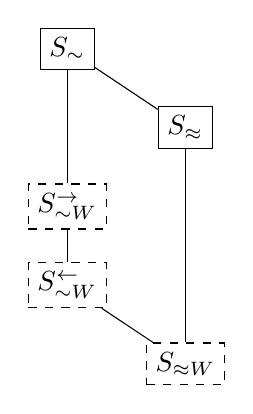
\begin{tikzpicture}
    \node (a1) at (0,4) [rectangle,draw] {$S_{\tyr}$};
    \node (a2) at (1.5,3) [rectangle,draw] {$S_{\tmr}$};
    \node (a3) at (0,2) [rectangle,draw,dashed] {$S_{\tyr W}^{\rightarrow}$};
    \node (a4) at (0,1) [rectangle,draw,dashed] {$S_{\tyr W}^{\leftarrow}$};
    \node (a5) at (1.5,0) [rectangle,draw,dashed] {$S_{\tmr W}$};
    \draw (a1) -- (a2);
    \draw (a2) -- (a5);
    \draw (a1) -- (a3);
    \draw (a3) -- (a4);
    \draw (a4) -- (a5);
  \end{tikzpicture}
  \caption{Hierarchy of Context Schemas}
  \label{fig:ctxschema}
\end{wrapfigure}

The schemas can be further arranged in a hierarchy (Fig.~\ref{fig:ctxschema}).
A context satisfying $S_{\tyr}$ can always be weakened to one sitting lower in the hierarchy.
The hierarchy also induces a strengthening relationship, going upwards, as long as subordination of prediactes/judgements under said contexts is respected.

%%% Local Variables:
%%% mode: latex
%%% TeX-master: "fscd17"
%%% End:


\section{Discussion and Observations}
\label{sec:disc-observ}

When we have to construct a proof for an intricate result, we are often tempted to just grab our favourite proof assistant and start hacking away.
While the approach may, with sufficient expertise, lead to a technically correct proof it is often the case that the end product does not reveal much more about the problem than ``the result holds''.
If we allow ourselves a moment of philosophical musing than we may recall that it is often claimed that the main purpose of a proof is to communicate, and convince, someone else that a certain fact follows from mutually accepted assumptions.
In this regard, all we have achieved so far is to convince some machine of such a fact.
In order to communicate the result to our colleagues as well, we usually need more than just a proof script or proof term -- we need intuitions.


\section{Conclusion and Outlook}
\label{sec:conclusion}

\subsection{Future Work}
\label{sec:future-work}

The results and observations obtained here are already interesting in their own right.
As a benchmark, however, they are only of a preliminary nature.
Thus we would like to extend the present work in at least two directions.

Firstly we would like to cover additional frameworks in order to see how well these are able to handle the present challenge.
Those of immediate interest are the so-called locally nameless techniques~\cite{DBLP:conf/popl/AydemirCPPW08} and the HYBRID framework~\cite{Capretta2007, Capretta2009, DBLP:journals/jar/FeltyM12}.
The locally nameless approach provides an abstraction layer that can be seen as sitting between the pure and low-level de Bruijn approach on the one hand and the high-level HOAS approach on the other.
The HYBRID framework for Coq, on the other hand, is in spirit very close to Abella and provides a HOAS layer for Coq.
It does, however, lack Abella's $\nabla$ and neither is it equipped with Beluga's capabilities of fine-grained contextual reasoning, so it remains to be seen if the framework is capable of dealing with our benchmark.
Should it turn out that HYBRID is not (yet) up to the task, then our benchmark could act as a useful guideline for future development.

The other direction we would like to focus on concerns the benchmark itself.
At the moment, we only look at the equivalence of the typability problem.
Note, however, that we are dealing with computational systems, and as such their reduction behaviours are at least as interesting as their typability problems.
Equi-reducebility will likely present its own set of challenges, as the PTS has many more $\beta$-redices, at least prior to typing.
And reduction is of course usually defined independent of typing.

Finally it would be interesting to formulate the whole setup not only for System~F, but also for the simply typed $\lambda$-calculus on the one hand and F$_\omega$ on the other.
For the remaining corners of Barendregt's $\lambda$-cube, like for example the calculus of constructions, no corresponding two-sorted variants exist.
It is thus unclear what a suitable benchmark would look like.


% \subparagraph*{Acknowledgements.}

% I want to thank \dots

% \appendix
% \section{FOO}

% Needed?



%%
%% Bibliography
%%

 \bibliography{ref,bp-extract}

\end{document}

%%% Local Variables:
%%% mode: latex
%%% TeX-master: t
%%% End:
